\documentclass[10pt,a4paper,headinclude=true]{report}
\usepackage[latin1]{inputenc}
\usepackage[a4paper]{geometry}
\usepackage{amsmath}
\usepackage{amsfonts}
\usepackage{amssymb}
\usepackage{graphicx}
\usepackage{hyperref}
\usepackage{pdflscape} % dlia landscape orientation 
\hypersetup{colorlinks,citecolor=black,filecolor=black,linkcolor=black,urlcolor=black}
\usepackage{float}
\usepackage{setspace}

%\usepackage{biblatex}

\renewcommand{\familydefault}{\sfdefault}

\begin{document}
\onehalfspacing
\title{Industrial Year placement report}
\author{Edgar Ivanov\\ edi@aber.ac.uk \\ \\ IY ICT \& Media Technician}
\date{\today}

\maketitle
\tableofcontents

\chapter{Organization}
Assume we know nothing \& take a funnel approach. Start broad i.e. brief history \&
size of university, how it is distributed, no. of departments, IS structure, your
team within IS, your place within the team.

My industrial year employment took place at Aberystwyth University, in Information Services department. Aberystwyth University is an institution of higher education with research departments, which provides undergraduate and postgraduate education. AU is located in small Aberystwyth town, on the west coast of Wales, with average population of 15 thousand people. University was founded in 1872 as University College Wales and changed its name since then a few times \cite{History}.
There are 17 academic departments and 27 service departments \cite{Departments} \cite{Departments2}. Most teaching departments are located on Penglais campus, as well as in Llanbadarn campus within 15 min walk from Penglais and in Old College where Welsh History department and managerial staff is located. There is as well big research department called IBERS (Institute of Biological, Environmental and Rural Sciences), it used to be independent organization but then was joined to AU. It is located in Gogerddan campus seven miles away from Penglais, so when I had jobs there I was using car. At this time there are plans to move some departments to Llanbdarn campus, which was hardly used in past years, so university will be even more spread across different locations.

\section{Information Services}
Information Services department is located in Hugh Owen Building and takes over 40 \% of E floor. Figure ~\ref{fig:isfloorplan} shows IS floor plan. Most of the IS staff are based in open plan office, with team leaders located in offices at the edges. Mine workplace was in workshop, which is a separate area from the main office. In the workshop there are eight people working on permanent basis, one Graduate Trainee who joined us in January for one year fixed contract and two IY's.

\begin{figure}[H]
\centering
\centerline{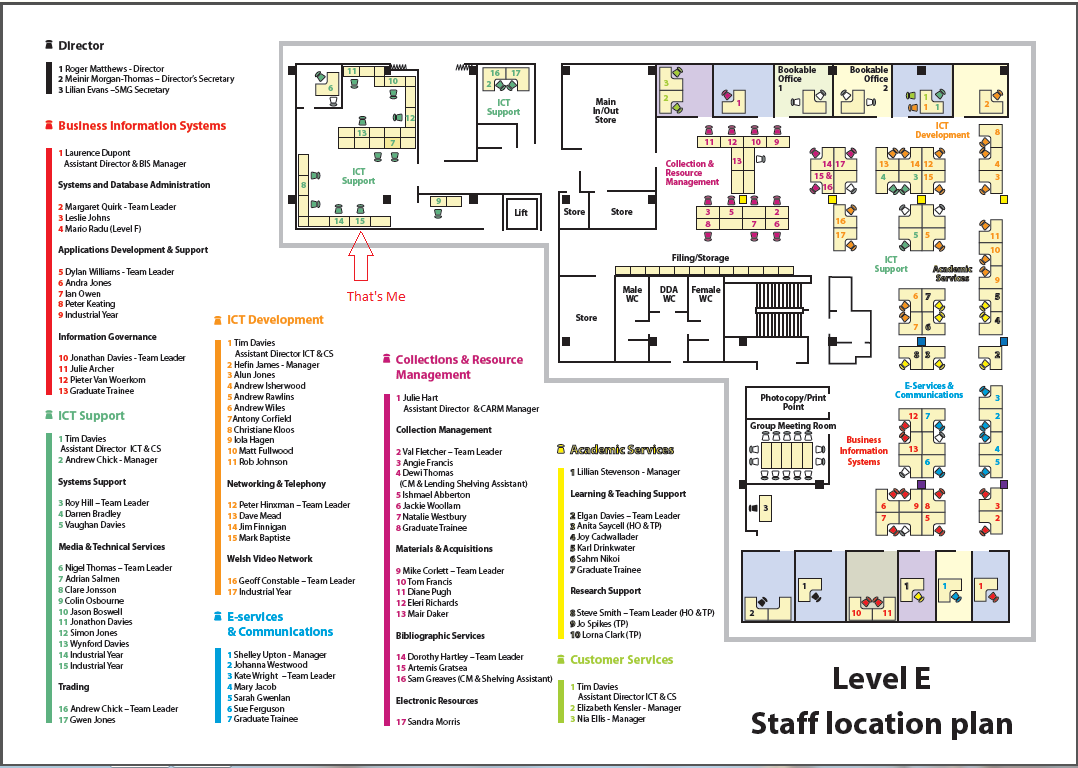
\includegraphics[scale=0.55]{./isfloorplan}}
\caption{IS Floor Plan \cite{ISFloor}}
\label{fig:isfloorplan}
\end{figure}

On figure~\ref{fig:i-s-hierarchy-tree-march-2012} you can see IS hierarchy tree.

\begin{figure}[H]
\centering
\centerline{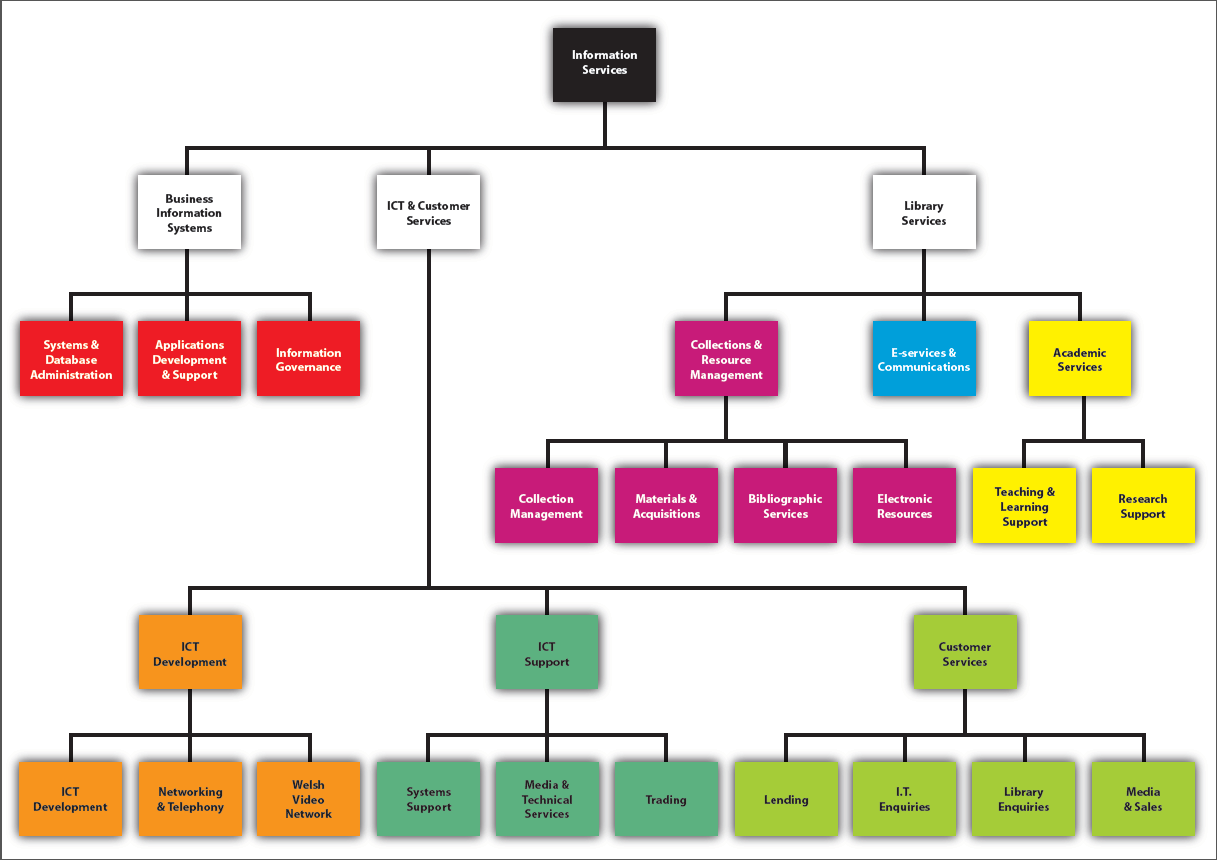
\includegraphics[scale=0.55]{./i-s-hierarchy-tree-march-2012}}
\caption{IS hierarchy tree}
\label{fig:i-s-hierarchy-tree-march-2012}
\end{figure}

\section{ICT Support}
\subsection{Media \& Technical Services}
The group that I am based in falls under IS $>$ ICT \& Customer Services $>$ ICT Support and is called "Media \& Technical Services". It is defined as a group responsible for the software and hardware upgrades and repairs a wide variety of ICT equipment types. It also provides multimedia services and supports ICT equipment within teaching spaces. This means that all computer relevant hardware repairs are done within this group, it includes internal repairs (the equipment owned by university) as well as repairs for external customers (staff, students, members of publicity). The members of this group also provide technical support to lecturers who are teaching and experience any issues with teaching equipment.

\subsection{Systems Support}
This group is responsible for all the aspects of PSV workstations, including software licensing, purchasing, management and implementation for Information Services and many departmental products. It makes backups for most of the University's systems and maintains two main server rooms, one in Penglais and one in Gogerddan. It also provides second/third line software support for the help-desk/workshop.
\subsection{Trading}
Offers a wide range of computers, laptops, media equipment and peripherals for sale to University Departments, individuals and external customers. Prices are generally competitive and are often at specially negotiated educational terms and/or with extended warranties for the members of the University,
\section{ICT Development}
Designs and implements systems and services for IS, other University departments, and external bodies. Also develops, implements, trains and supports IS users on bespoke software and ensures existing systems are efficient and cost effective. This includes Network and Telephone service design promoting standardization and centralization and managing improvements and information security incidents.
\section{Customer Services}
Provides Lending, ICT enquiries, Media \& Sales and Library Enquiry services for staff, students and visitors. Monitors the responsiveness and effectiveness of front-line services, ensures services best meet users' needs and promotes awareness of IS enquiry and front-line services. It also manages services and staffing for Freshers' Weekends and students' induction programmes.

\subsection{I.T Enquiries}
I will give more details on I.T Enquiries group, where other IY's are based, since I work a few hours a week in this group as well as working for the Media and Technical services.

The first point of contact for face-to-face and online IT enquiries for all Information Services users. Troubleshoots any problems users experience with accessing or using Information Services services and resolves them or refers them as appropriate. Also supports the Public printing service, facilitates access to Information Services services such as email accounts, Aber cards, computing network, and printing and represents our users within IS e.g. presenting user feedback at meetings or user testing new services. I did two shifts a week on Service Point 2, helping customers with technical enquires and directing .

\section{BIS and Library Services}
There are also two other main groups called "Business Information Systems" and "Library Services". People in BIS are  responsible for development and support of the systems and processes required to maintain Admissions, Student Records, Finance, HR, Payroll and other associated business functions of the University. Library Services looks after all education materials: books, journals, articles as well as after education software systems like blackboard.


\section{People that I worked with}


\chapter{Technical environment}
When I just started my placement I was frustrated with amount of different software used in IS and how information was spread across all these systems. At the beginning I was introduced to Interzone, Sunrise, Astra, Recall, SharePoint, Aber FAQs, Outlook, Voyager. All used to store different kind of information. 

\section{Criticism}One of the issues I found that if I wanted to find some procedures I would need to check Sharepoint as well as Aber FAQs, since I could find what I need on any of this systems. Information about data projectors in teaching rooms is kept on SharePoint in simple Excel spreadsheet, which can be altered by anyone. Computer room layout with computer serial numbers kept on one of the employees M drive and is accessible through the web. So if Clares account will be locked for some reason, non of the workshop members will be able to access that data. Good example is PSR2 maintenance application which was clearly written by Clare for herself to make her job easier. On figure ~\ref{fig:main_PSR2_page} you can see main PSR2 page, which contains some teaching rooms list that workshop technicians looks after.

\begin{figure}[H]
\centering
\centerline{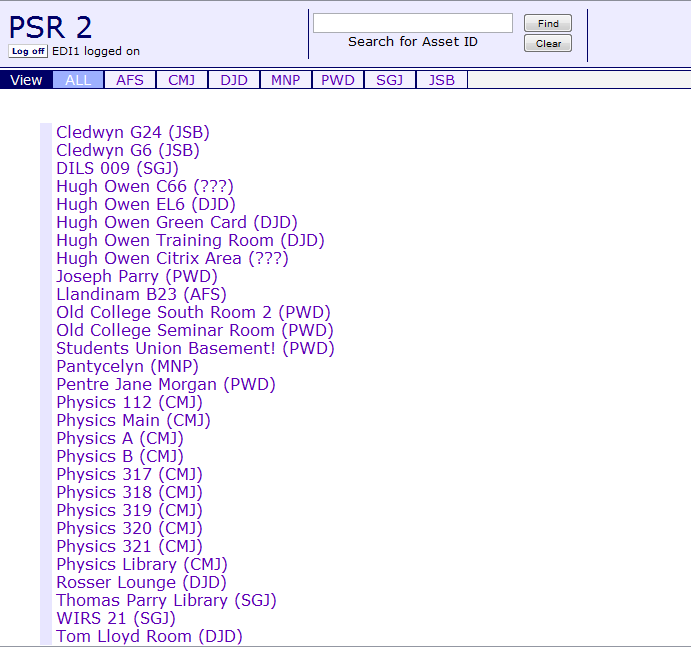
\includegraphics[scale=0.3]{./PSR2}}
\caption{Main PSR2 Page}
\label{fig:main_PSR2_page}
\end{figure}

Figure~\ref{fig:PSR2_SU_Room_layout} shows Students Union computer room layout, with computer names and serial numbers. Room comment holds code to unlock monitors from security straps. It also contains information when each computer was last time checked. So it contains quite a lot of information, which is crucial to our work, and if for some reason Clares account will be locked or she leaves university we will loose access to that information, which is not held any where else.

\begin{figure}[H]
\begin{center}
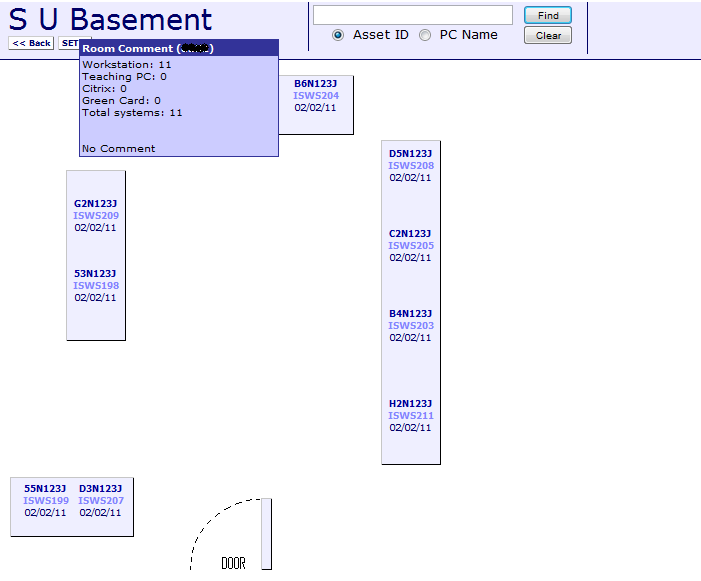
\includegraphics[scale=0.5]{./PSR2_SU_Room_layout}
\caption{PSR2 Students Union Computer Room Layout}
\label{fig:PSR2_SU_Room_layout}
\end{center}
\end{figure}


\section{Interzone}
Interzone is a front end web interface for the database that is used to manage records of network equipment in Aberystwyth University. On the main page you can search for record that contains specified information in it. It is possible search by IP address, MAC address, Owner's login, computer name etc. On the figure ~\ref{fig:main_interzone_page} you can see main Interzone page.

\begin{figure}[H]
\centering
\centerline{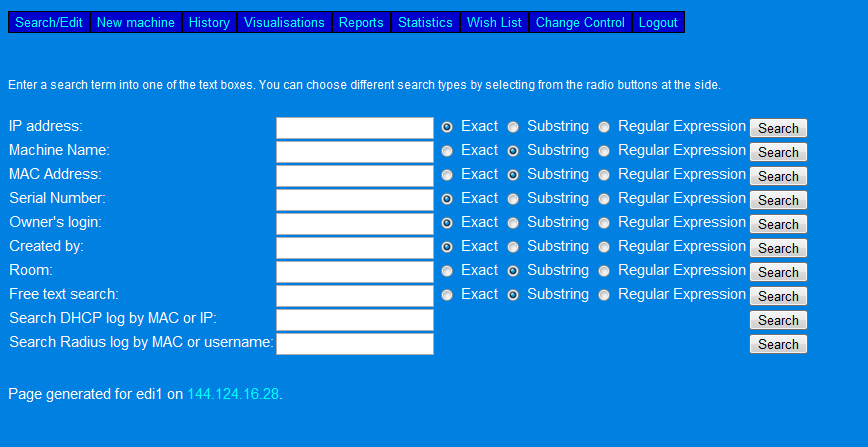
\includegraphics[scale=0.5]{./main_interzone_page}}
\caption{Main Interzone Page}
\label{fig:main_interzone_page}
\end{figure}

On figure ~\ref{fig:machine_record} you can see Interzone record of my computer.

\begin{figure}[H]
\centering
\centerline{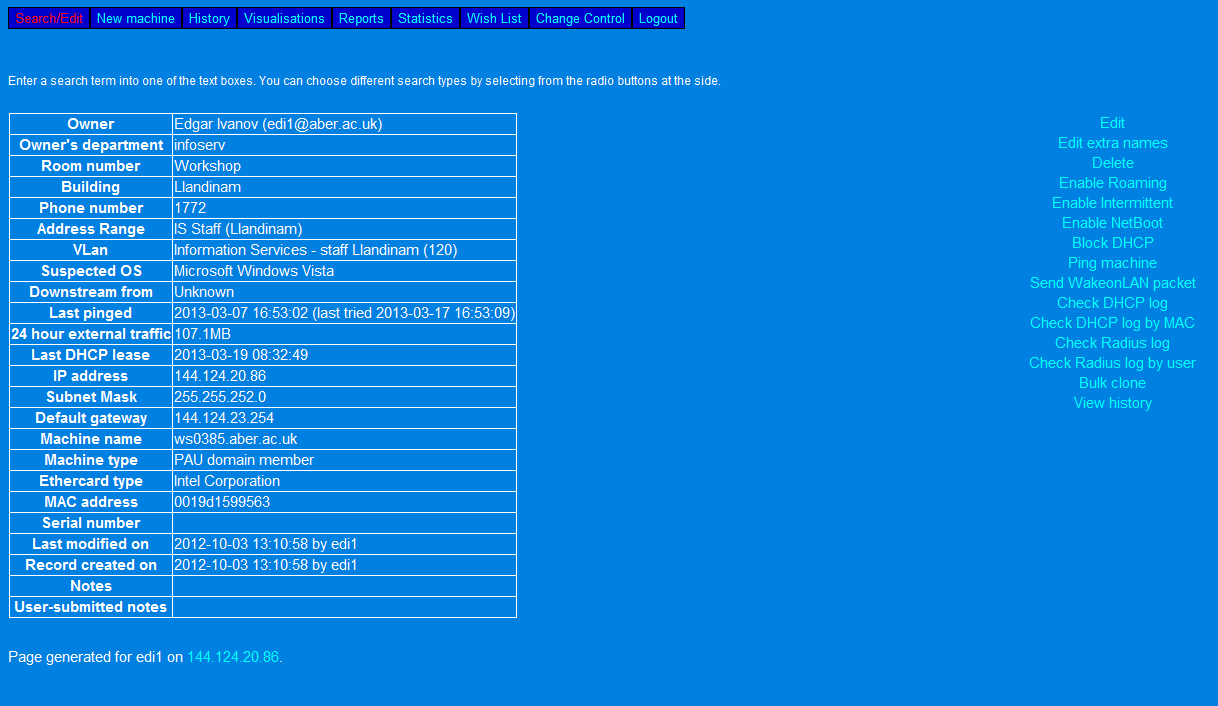
\includegraphics[scale=0.5]{./machine_record}}
\caption{Machine record}
\label{fig:machine_record}
\end{figure}

It contains various information about the owner, owners department, telephone number (if there is one), VLAN, IP and MAC addresses, you can also see who created this record and when it was last modified.

\begin{figure}[H]
\centering
\centerline{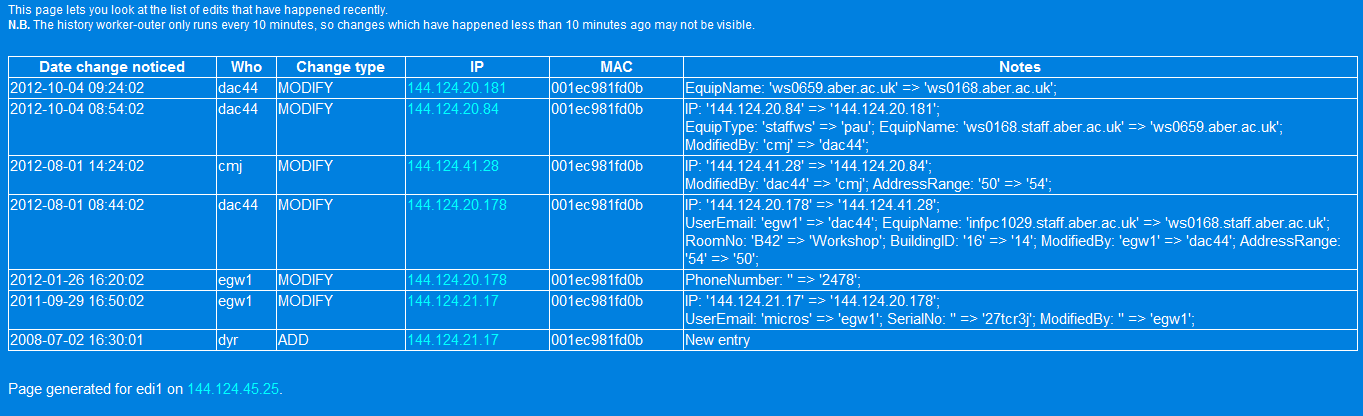
\includegraphics[scale=0.5]{./modification_history}}
\caption{Modification History}
\label{fig:modification_history}
\end{figure}

Information gathered from interzone can be very useful when troubleshooting computer connection issues. It is possible to check DHCP log to see if computer gets IP address, look at the RADIUS logs that contain information if the user was successfully in authenticating in out system or not. Figure ~\ref{fig:interzone_radius} shows RADIUS log for my mobile phone, where it is clearly seen that at some point in time I was unable connect to the network due to the authentication problems. When working on help desk and troubleshooting somebody's device, which was not connecting to the internet or not working properly, Interzone logs let me know what was going wrong so that I could choose appropriate solution.

\begin{figure}[H]
\centering
\centerline{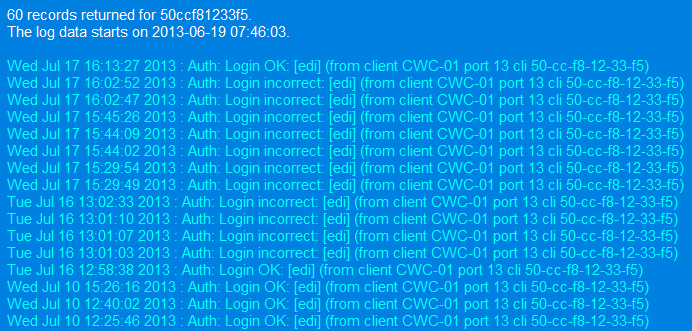
\includegraphics[scale=0.5]{./interzone_radius}}
\caption{RADIUS log}
\label{fig:interzone_radius}
\end{figure}

\section{Sunrise}
Sunrise is another front end web interface for the database that we use to keep track on current and past calls. It lets us to create new jobs, assign them to the technicians, add comments about the job, send emails to the user etc. On the figure ~\ref{fig:sunrise_main} you can see main Sunrise page, with all open and assigned to me jobs as well as the boxes where you can specify search criteria and search for the specific job.

\begin{figure}[H]
\centering
\centerline{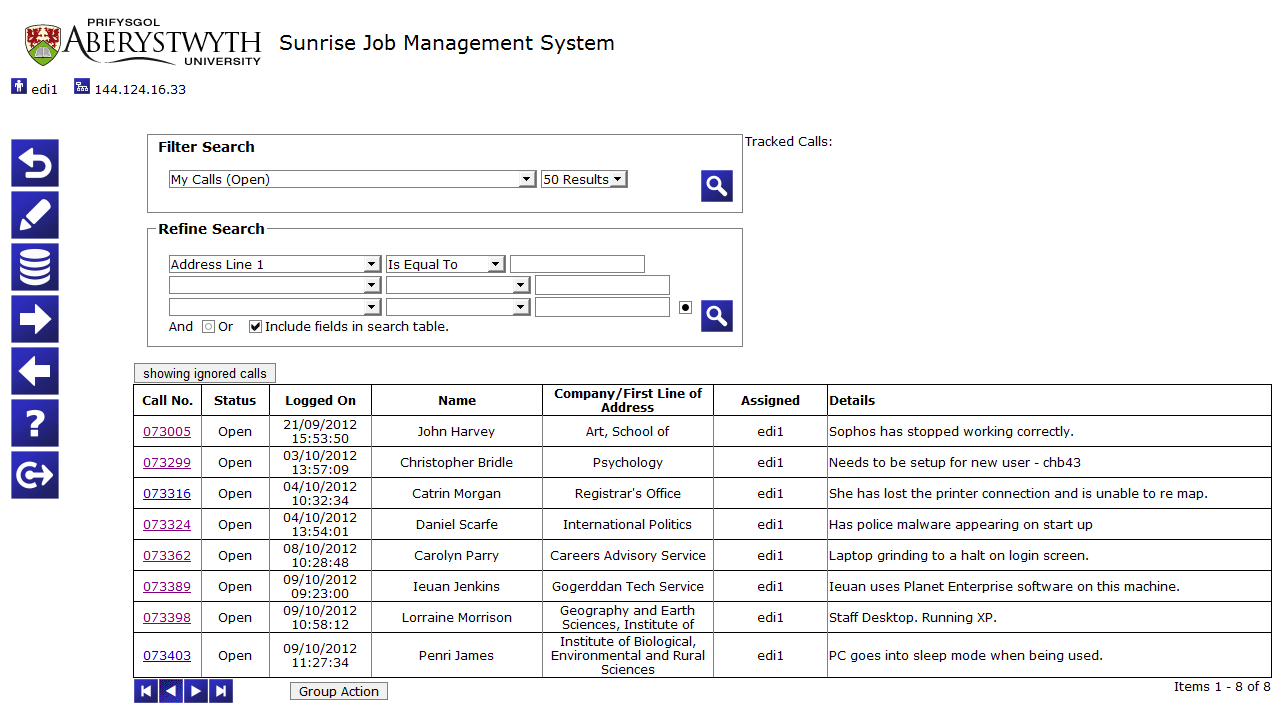
\includegraphics[scale=0.5]{./sunrise_main}}
\caption{Sunrise Main Page}
\label{fig:sunrise_main}
\end{figure}

On the figure ~\ref{fig:sunrise_search} you can also see all the jobs that contain my email address ?edi1? in them.

\begin{figure}[H]
\centering
\centerline{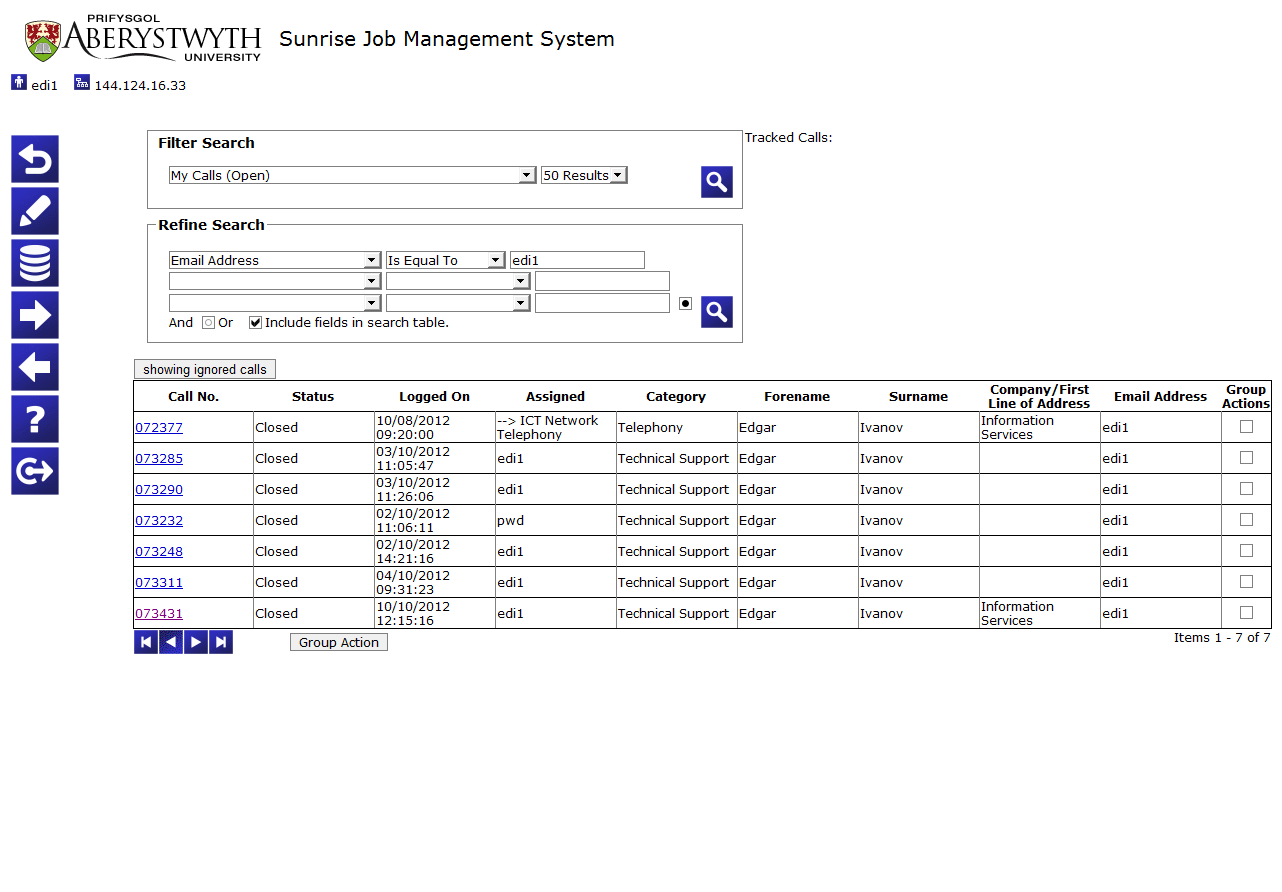
\includegraphics[scale=0.5]{./sunrise_search}}
\caption{Sunrise Search}
\label{fig:sunrise_search}
\end{figure}

Figure ~\ref{fig:sunrise_job} represents an ordinary job. Each job has a unique Call Number, in this case it is 075028, it also has the email address of the person who this job was opened for, phone number, address, equipment serial number, equipment description (laptop, desktop PC, projector, printer) and comments where a fault or an issue is described. On the right hand side you can see job history pane, each action that technician does must be added to the history so that if there will be any questions or issues in future it is possible to see what was done.

\begin{figure}[H]
\centering
\centerline{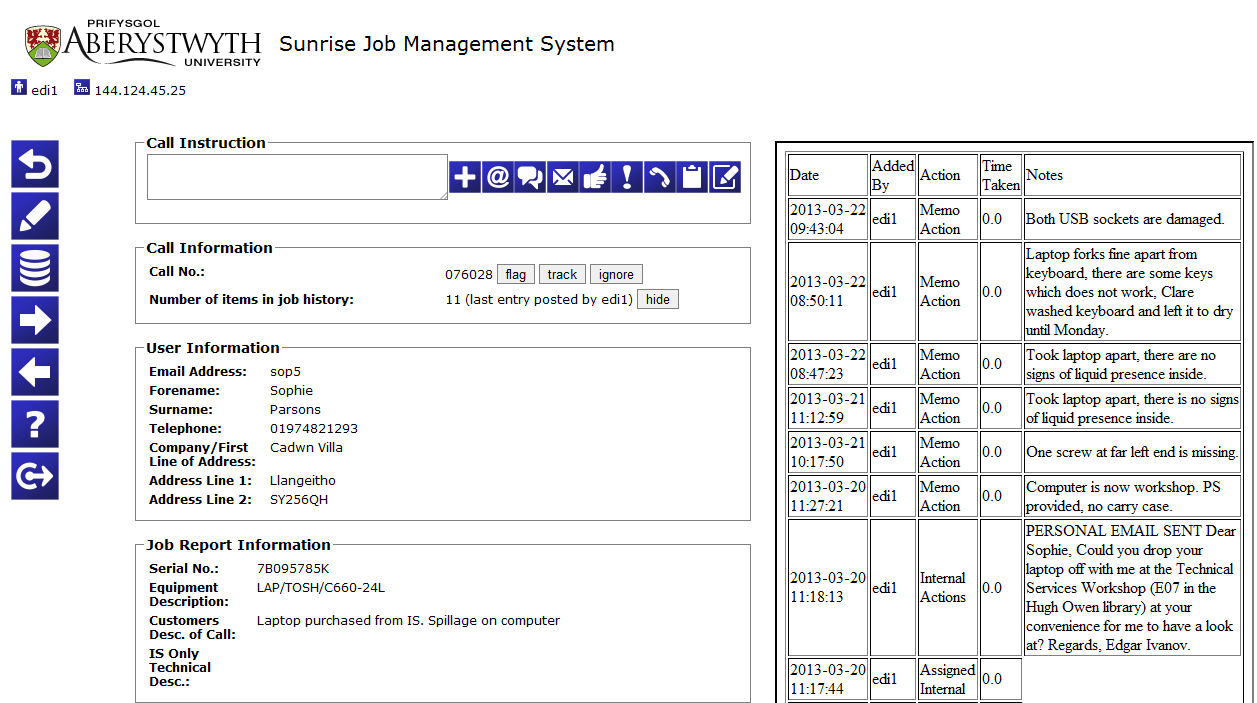
\includegraphics[scale=0.5]{./sunrise_job}}
\caption{Sunrise Job Record}
\label{fig:sunrise_job}
\end{figure}

\section{SNMPc network manager}
Aberystwyth University is a large organization, having thousands of devices connected to its network. To provide reliable service for end users we need to ensure that our network functions properly and issues are fixed as soon as possible. Network equipment such as: computers, printers, IP cameras, SALTO locks, wireless access points, VoIP phones all relay on ability to communicate (send/receive data), so it is crucial to ensure that there is working network connection at all times.  To monitor all our switches, routers, servers, workstations and printers IS uses program called SNMPc, developed by Castle Rock Computing. SNMPC is a Distributed Network Manager \cite{SNMPc} that uses SNMP protocol which stands for Simple Network Management Protocol. SNMPc makes it easier to look after whole network and network devices by identifying unresponsive equipment or path with the issues. Figure ~\ref{fig:SNMPc_main} shows map of our network. Green or purple icon shows that all pollable nodes in them are contactable. If icon turns red it indicates that at least one node in this sub map is not contactable any more \cite{SNPMcSharePoint}. Buy just looking at the map it is possible to identify if there are any issues on the network and if there are try to fix them. I didn't use this application much since there are other people responsible for keeping our network up and running, but I found it quite interesting and useful to look at it time to time since I could see and explore our network in graphical view.

\begin{figure}[H]
\centering
\centerline{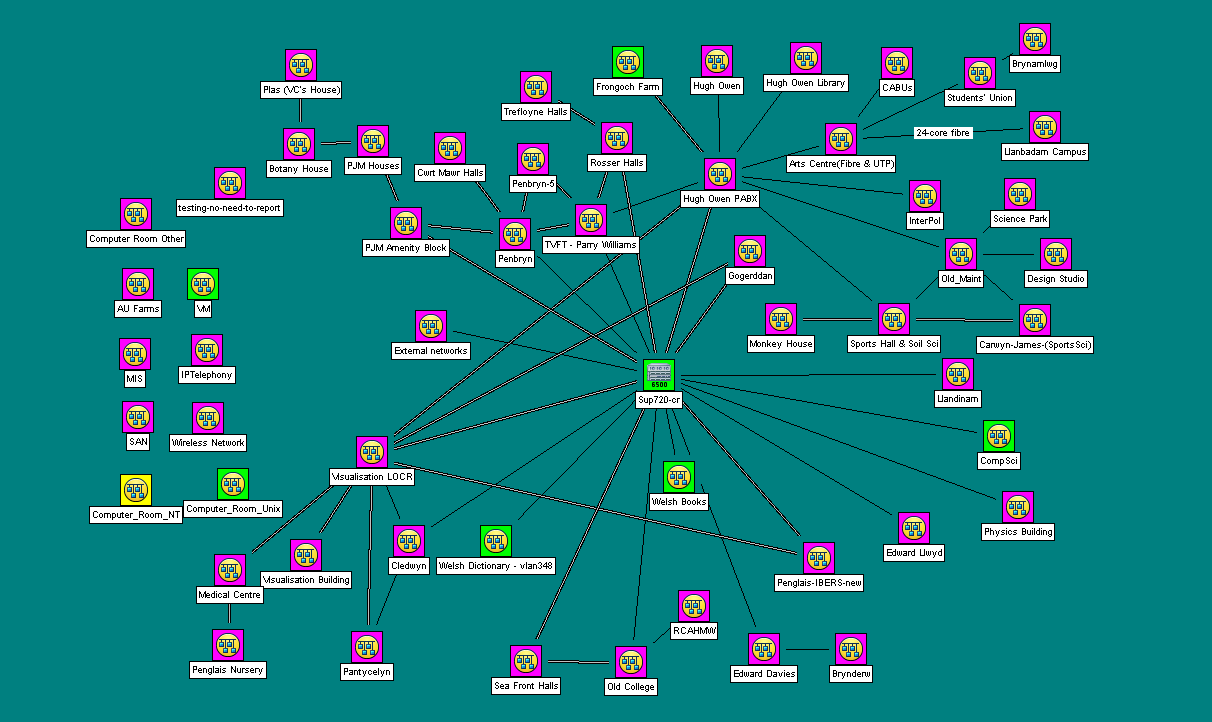
\includegraphics[scale=0.5]{./SNMPc_main}}
\caption{University network map in SNMPc application}
\label{fig:SNMPc_main}
\end{figure}

\section{VoIP Phones}
\section{Public Workstation Computers}
Public Workstation Computers are computers that can use anybody who have university account. IS manages around 500 public computers across campus. This summer we deployed new USFF Dell Optiplex 7010 \cite{PSVs} computers. We have two different versions of Optiplex 7010 computers. One model with higher specifications for teaching stations and USFF model for student use. All our PSVs run MS Windows 7 OS, there are more than 200 applications installed for academic use on them. PSV computers are configured to wipe everything straight away from "C" drive after user logs off, exception is only "D" drive where data is wiped every five days. Consequence of that is if somebody forgets to save document on USB pen drive or somewhere else and logs of from the computer they will lose data. This year senior management decided to change this and all user files will be redirected automatically to "M" drive, all standard Windows folders such as "My Document", "Pictures", MS Office auto save path etc. (on-line storage provided to everybody in university who has computing account, size is usually limited to 2 GB per user. This on-line storage is usually mapped automatically when user logins on to the computer).

\begin{figure}[H]
\centering
\centerline{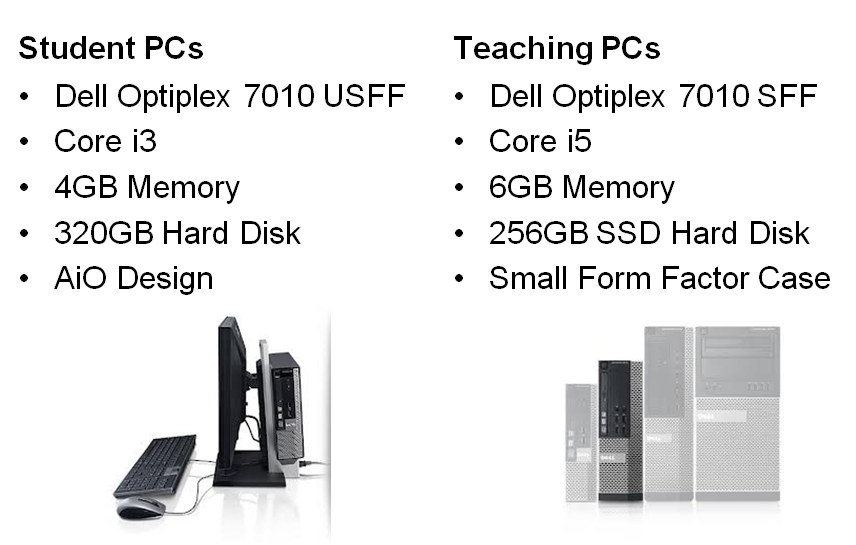
\includegraphics[scale=0.5]{./PSVs}}
\caption{Public workstation PCs \cite{PSVs}}
\label{fig:PSVs}
\end{figure}

\section{REG}
Whenever somebody becomes part of the university(staff, students) there is university account created for them consisting from three letters and some digits if required, mine for example was "edi1". Users then can use them to access their emails, e-journals, manage records about themselves and login to all the systems in university (if they have access to them of course). To manage these accounts we have web interface called REG. I was using it mainly for unlocking user accounts while working on help desk, issuing new passwords, verifying identity of the people coming to the desk. On of the options I had was to make temporary password for any user, so that I could login as them to any system. It was quite useful when I needed to migrate user profile folder on Windows OS and user was away or it was not feasible for them to come in workshop. In such cases I would create temp password, login on the computer as them (that is when Windows creates actual folder for the user on the computer together with other corresponding registry entries), log off and revert password back, after all these step I could copy all files from one machine to another and be sure that everything will work after user will login on to their machine.
\section{Computers}

\section{Pcounter}
PCounter is an application that allows to  manage user print profiles. It allows to see print balance for everybody in university, it is possible to increase or decrease balance on the account, see print history and produce reports. I used it mainly for adding money to the user accounts when print credit machine was broken and users were coming to the desk to top up their account.

\section{Workshop technical environment}
Computer Workshop Technical Environment is probably most unusual in comparison to the rest of IS. Here we not only deal with software related issues, but a hardware as well: soldiering, computer part replacement, cleaning after spillages, equipment shifting.
When term starts we tend to get quite a lot of laptops that fail to boot in to OS. Usually it is caused by damaged HDD having broken sectors that can not be red by running software. In such cases disk cloner becomes extremely useful since it can skip broken sectors, filling them with zeros on destination drive making it possible to copy at least some data from working copy.

We also tend to get requests to restore lost data. In such case we use R-Studio program which performs scan o whole drive and then displays all data that is available for recovery.

Symantec Ghost this is application that we use to make one-to-one copy of HDD or just one partition of it. It is possible to store copy as an image file as well. It is heavily used during new version of Windows deployment on Public Workstation computers. After reference Windows installation is complete and all necessary programs are installed, whole HDD is being copied in to the file as is, afterwards PSV computers join multicast session and image captured before is applied to all of the machines. It is very nice technique sine there is no need to spend hours at each computer installing Windows with all corresponding applications required for education needs. Taking in account that new updates are released almost weekly we make new reference image every year and deploy it over the summer when computers are not in great use. In public use around campus there are almost 500 (?) computers, so deploying windows on 60 computers in 3-5 hours is really good achievement.

Winternals Administrator Pack is a collection of tools released  by (Microsoft or Mark russinovich?), form this pack I used only Active Dirctory Explorer and XXXXXXX to see what connection computer makes.
  
\chapter{What I did}
Describe your 'routine' weekly duties. Spend a bit more time on areas where you have
responsibility or have put in effort e.g. summer builds, FAQS, summer course
registrations, any exploratory projects or mini-projects you may have been given to
name a few.

\chapter{Critical evaluation}
\bibliographystyle{ieeetr}
\bibliography{bibl}

\end{document}